\documentclass[10pt]{article}
\usepackage[polish]{babel}
\usepackage[utf8]{inputenc}
\usepackage[T1]{fontenc}
\usepackage{amsmath}
\usepackage{amsfonts}
\usepackage{amssymb}
\usepackage[version=4]{mhchem}
\usepackage{stmaryrd}
\usepackage{graphicx}
\usepackage[export]{adjustbox}
\graphicspath{ {./images/} }

\title{GIMNAZJUM }

\author{}
\date{}


\begin{document}
\maketitle
\begin{enumerate}
  \item W butli jest 12 litrów wody. Połowę zawartości butli trzeba przelać do pustego naczynia, ale do przelewania możemy użyć tylko naczyń o pojemności 8 litrów i 5 litrów. Jak to zrobić?
\end{enumerate}

\section*{2. Do okręgu należą kolejne punkty A, B, C, D. Kąt środkowy}
oparty na łuku BC ma miarę \(\alpha\), a kąt środkowy oparty na łuku AD ma miarę \(\beta\). Wyznacz miarę kąta, pod jakim przecinają się odcinki AC i BD.\\
3. Wykaż, że jeżeli pewną liczbę można przedstawić jako\\
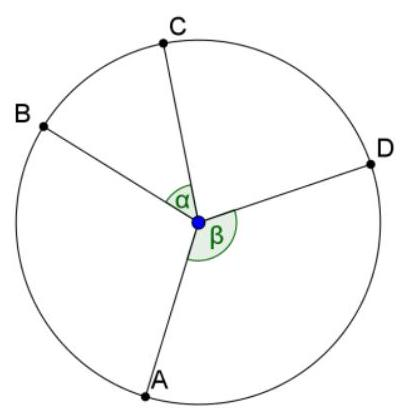
\includegraphics[max width=\textwidth, center]{2024_11_21_8d452c3074d21c805645g-1}\\
sumę kwadratów pewnych dwóch liczb naturalnych, to również jej dwukrotność można przedstawić w postaci sumy kwadratów dwóch liczb naturalnych.

\section*{LICEUM}
\begin{enumerate}
  \item W wiadrze jest co najmniej 10 litrów mleka. Czy można odlać z niego dokładnie 6 litrów, posługując się dwoma naczyniami o pojemności odpowiednio 9 i 5 litrów?
  \item Dany jest trójkąt \(A B C\), w którym kąt \(A B C\) ma miarę \(60^{\circ}\). Wykaż, że punkty A i C oraz ortocentrum i środki okręgów wpisanego i opisanego na trójkącie \(A B C\) należą do jednego okręgu.
  \item Wykaż, że jeżeli pewną liczbę można przedstawić jako sumę kwadratów pewnych dwóch liczb naturalnych, to również jej trzynastokrotność można przedstawić w postaci sumy kwadratów dwóch liczb naturalnych.
\end{enumerate}

\end{document}